\documentclass[t,english]{sdqbeamer}
%\documentclass[c]{sdqbeamer}

\usepackage{listings}
\usepackage{graphicx}
\usepackage{tabularx}
\usepackage{tikzsymbols}
\usepackage{booktabs}
\usepackage[final]{pdfpages}

\usepackage[lined,linesnumbered,ruled,noend]{algorithm2e}
\renewcommand{\thealgocf}{}

\hypersetup{
	colorlinks=true,
	urlcolor=kit-green,
	citecolor=mygray
}

% set sdqbeamer options
\titleimage{blender-render}
\groupname{} % rendered at the bottom center of each slide
\grouplogo{ae+satres}
\selectlanguage{english}

% define title etc.pp.
\title{Practical SAT Solving}
\subtitle{Lecture 13 \unimp{\normalfont -- Maximum Satisfiability (MaxSAT)}}
\author{\underline{Ashlin Iser}, {Dominik Schreiber}}
\date{July 28, 2025}

% define commands
\input{l00-commands.tex}

%\usepackage[english]{babel}
\usepackage[citestyle=numeric,bibstyle=numeric,hyperref,backend=biber,language=auto]{biblatex}
\addbibresource{references.bib}
\bibhang1em
\setbeamertemplate{navigation symbols}{}

\setlength{\itemsep}{1em}


\begin{document}

\begin{frame}[title white horizontal, picture=logos/blender-render, kitlogo=rgb]
	\titlepage
\end{frame}


\begin{frame}{Maximum Satisfiability}
Today's lecture is based on the slides by Prof. Matti J\"{a}rvisalo presented at 2016 SAT Summer School.~\\[1em]

\begin{columns}
\begin{column}{0.3\textwidth}
\centering
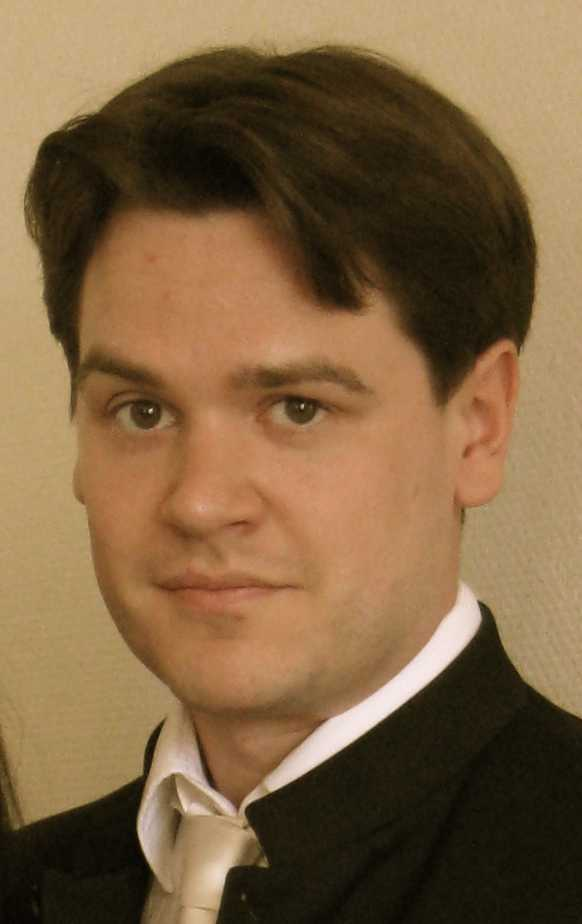
\includegraphics[scale=0.25]{figures/l13/jarvisalo.jpg}
\end{column}
\begin{column}{0.3\textwidth}
\centering
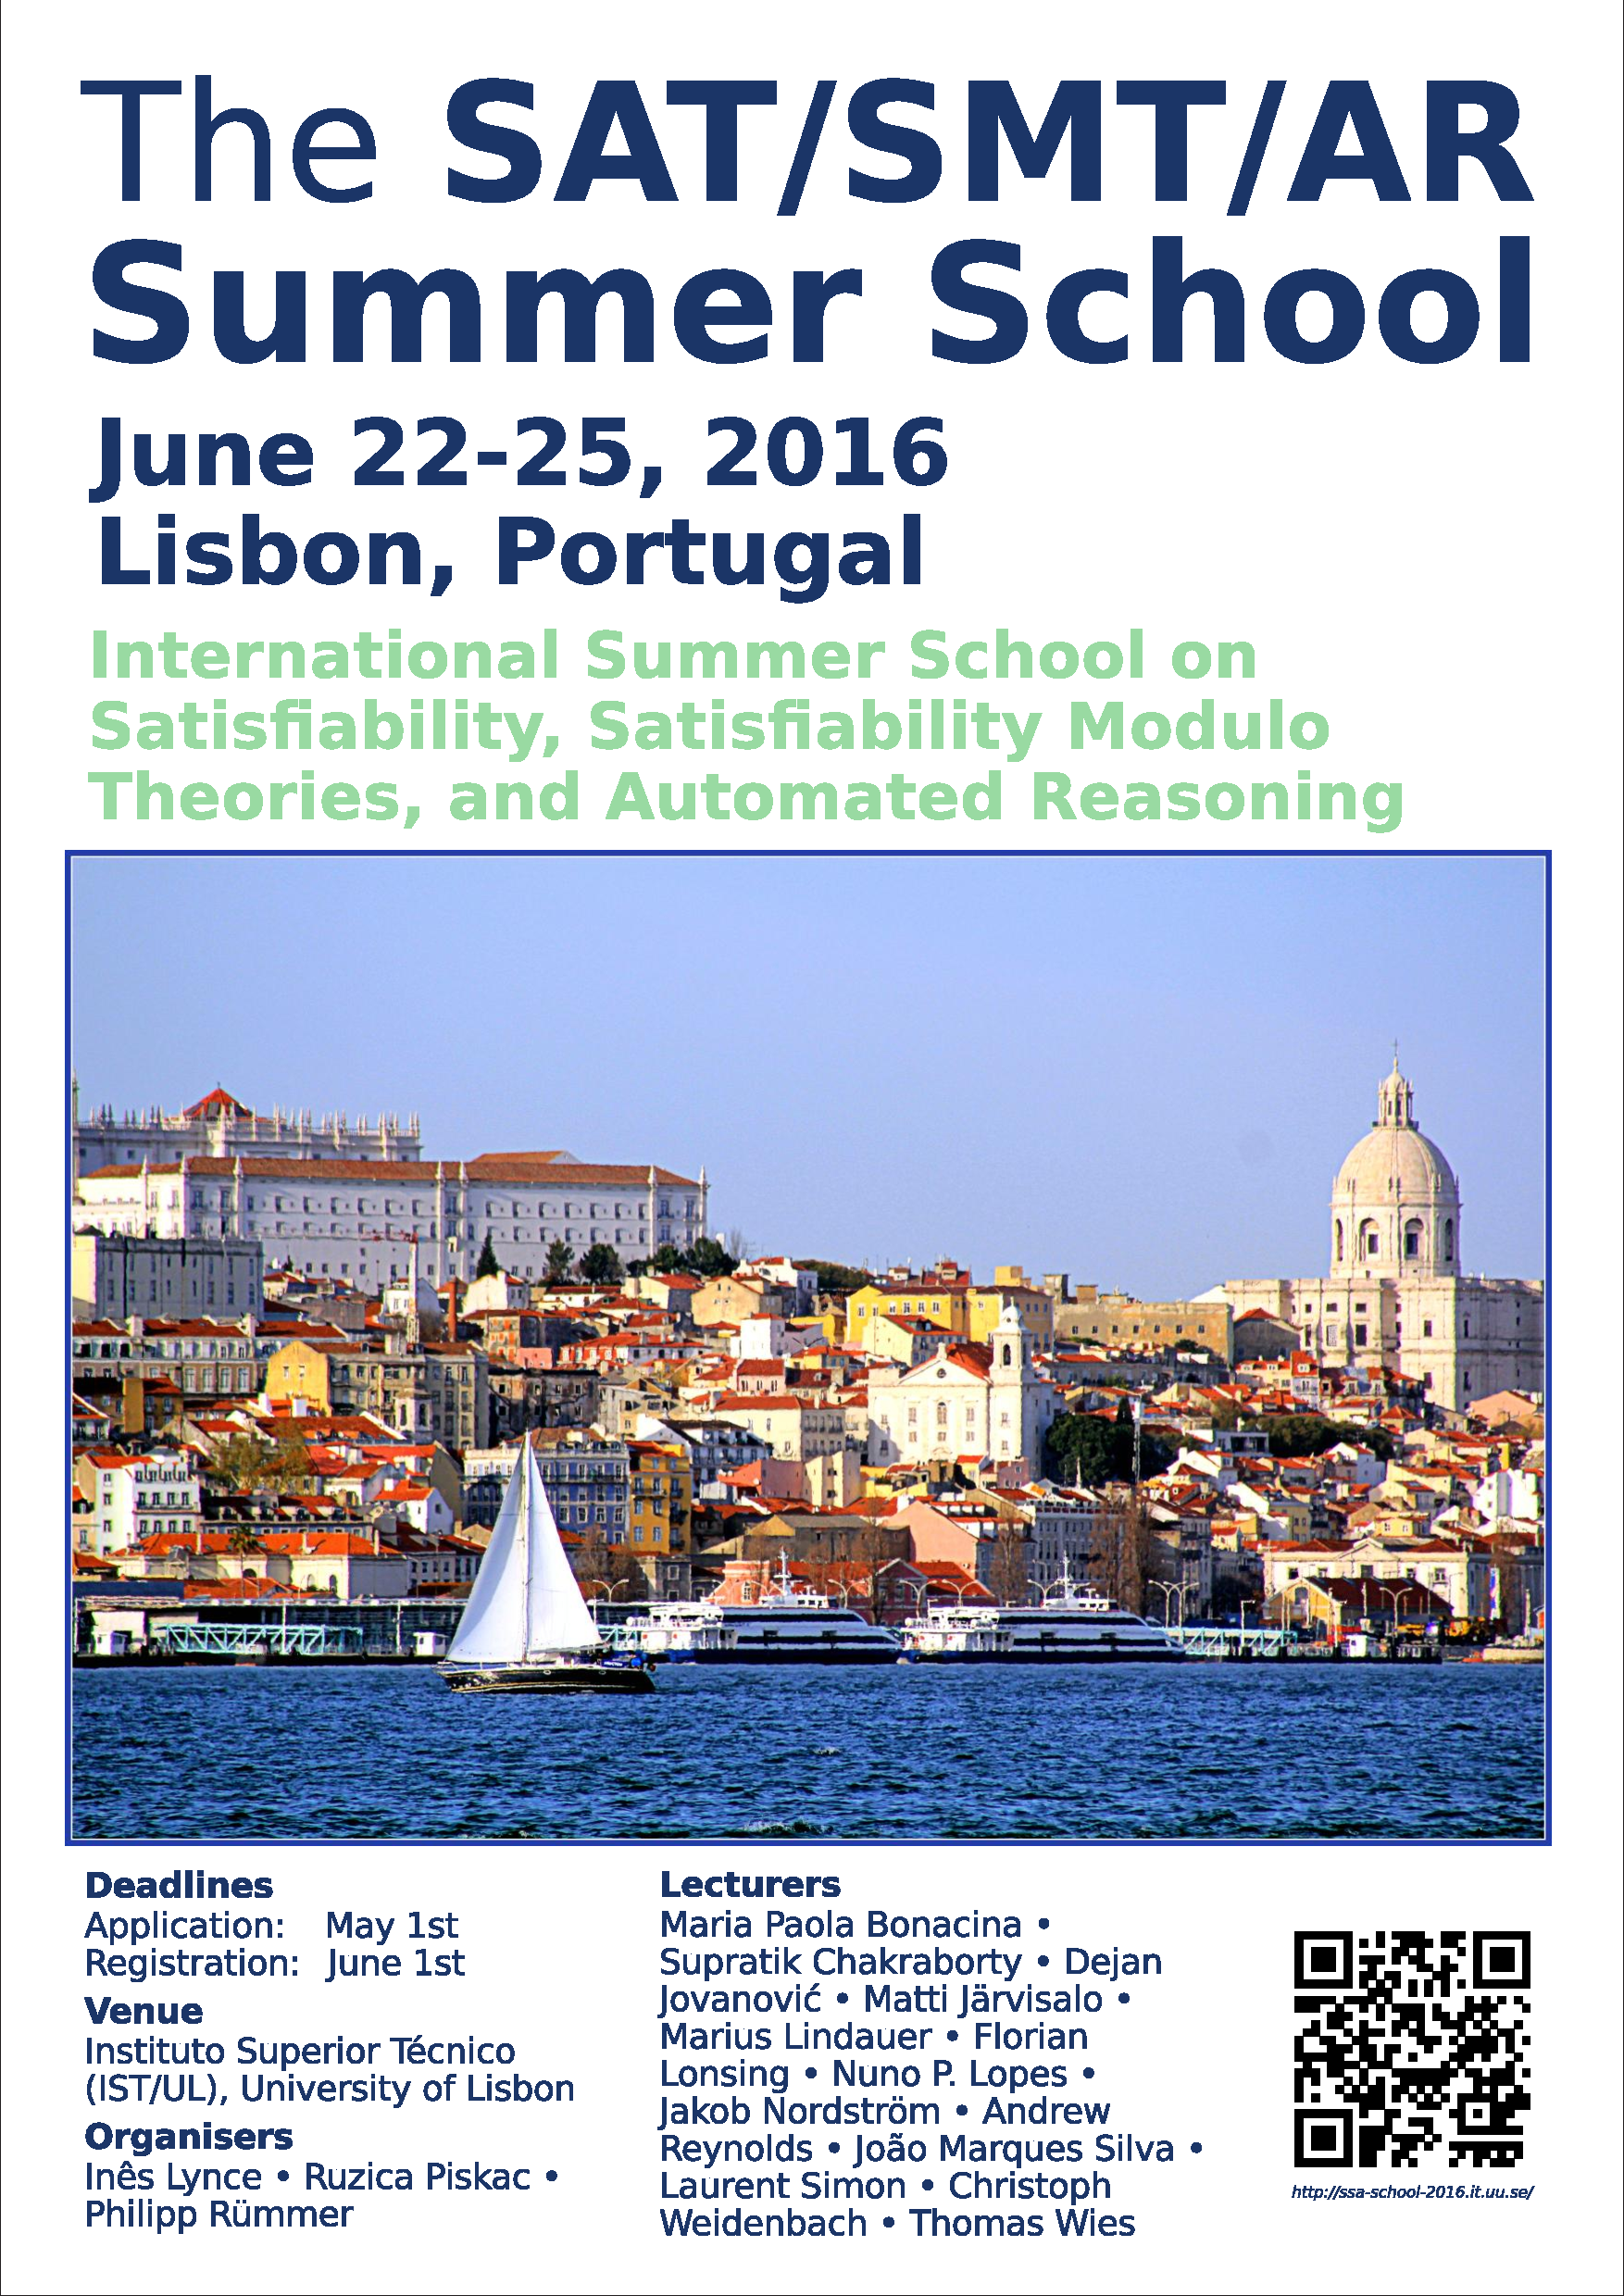
\includegraphics[scale=0.20]{figures/l13/ssa-poster-school.pdf}
\end{column}
\end{columns}~\\[1em]
\vfill
\hfill\url{http://ssa-school-2016.it.uu.se/programme/\#maxSAT}
\end{frame}

% {
% %\setbeamercolor{background canvas}{bg=\red}
% 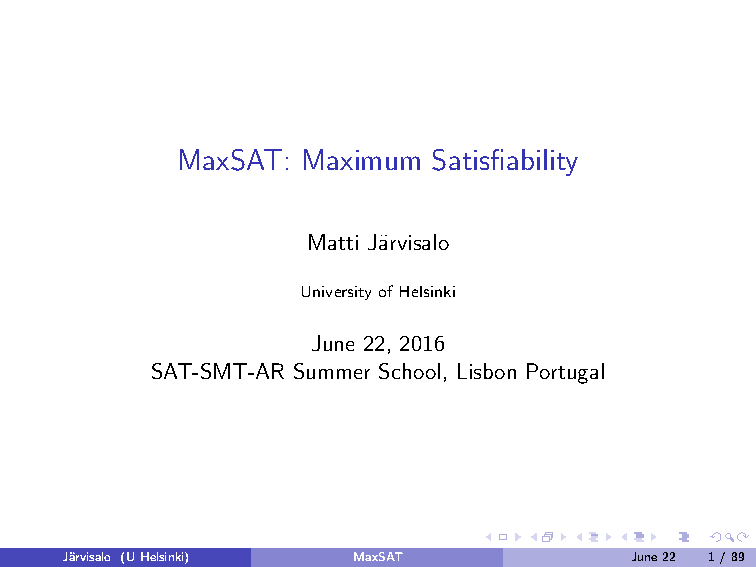
\includepdf[pages=1-]{l13-maxsat-matti.pdf}
% }

\begin{frame}{Maximum Satisfiability (MaxSAT)}{Exact Boolean Optimization Paradigm}
\begin{itemize}\itemsep1em
\item Basic concepts: MaxSAT, complexity, and applications
\item Overview of algorithmic approaches to MaxSAT\\[1ex]
	\begin{itemize}\itemsep1ex
		\item Branch and Bound
		\item Integer Programming (IP)
		\item Linear SAT-UNSAT (LSU) Approach
		\item Core-guided Approach
		\item Implicit Hitting Sets (IHS)
	\end{itemize}
\end{itemize}
\end{frame}

\begin{frame}{Boolean Optimization}{Motivation}
Most real-world problems involve an optimization component. There is a high demand for automated approaches to finding good solutions to computationally hard optimization problems.\\[1ex]
\begin{block}{Examples}
\begin{itemize}\itemsep1ex
	\item Find a shortest path/plan/execution to a goal/error state: \emph{Planning, model checking, debugging, \dots}
	\item Find a smallest explanation: \emph{Explainable machine learning, \dots}
	\item Find a least resource-consuming schedule: \emph{Scheduling, logistics, \dots}
	\item Find an optimal swap cycle in a kidney exchange: \emph{Healthcare}
\end{itemize}
\end{block}
\begin{block}{Benefits}
\begin{itemize}\itemsep1ex
	\item Resource savings (time, workforce, energy, material, \dots)
	\item Life savings (e.g., in healthcare, disaster response, \dots)
	\item Accuracy and proofs of optimality
	\item Better approximations by optimally solving simplified problem representations
\end{itemize}
\end{block}
\end{frame}

\begin{frame}{MaxSAT}{Classic Definition and Terminology}
\textbf{Input:} CNF formula $F$ (set of clauses)\\
\textbf{Task:} Find an assignment $\tau$ that maximizes the number of satisfied clauses\\[1ex]
\begin{block}{Central Generalizations}
\begin{itemize}
	\item \textbf{Weighted MaxSAT:} Each clause $C$ has a weight $w_C$, and the goal is to maximize the total weight of satisfied clauses.
	\item \textbf{Partial MaxSAT:} Some clauses are hard (infinite weight); only soft clauses can be violated.
	\item \textbf{Weighted Partial MaxSAT:} Mix of hard clauses and weighted soft clauses.
\end{itemize}
\end{block}
\begin{block}{Terminology}
\begin{itemize}
	\item \textbf{Solution:} Assignment satisfying all hard clauses
	\item \textbf{Cost:} Sum of weights of falsified soft clauses
	\item \textbf{Optimal Solution:} One that minimizes the cost
\end{itemize}
\end{block}
\end{frame}

\begin{frame}{Generic Linear Optimization Paradigms}
\vspace{-2em}
\textbf{Relationship with Generic Optimization:} Each MaxSAT instance can be reencoded such that all soft clauses are unit clauses. Soft unit clauses can then be interpreted as variables in an objective function of a generic optimization problem.~\\[1em]
\emph{Given a conjunction of constraints} $\bigwedge_k C_k$ of the form $C_k := \sum\limits_{i=1}^n c_{ki} x_i \leq b_k$ (with coefficients $c_{ki}$ and bound $b_k$),\\
\emph{find an assignment} to the variables $x_i$ that satisfies all constraints\\
\emph{and that maximizes} the objective function $\sum\limits_{i=1}^n c_i x_i$ (with coefficients $c_i$).~\\[1em]
\begin{block}{Constrained Optimization Paradigms}
\begin{itemize}\itemsep2em
	\item Maximum Satisfiability (MaxSAT)
	\begin{itemize}\itemsep1ex
		\item Variables $x$ are Boolean, Coefficients $c \in \{-1, 0, 1\}$, Bound $b=-1$
	\end{itemize}
	\item Pseudo-Boolean Optimization (PBO)
	\begin{itemize}\itemsep1ex
		\item Variables $x$ are Boolean, Coefficients $c$, and Bound $b$ are Integers
	\end{itemize}
	\item Integer-Linear Programming (ILP)
	\begin{itemize}\itemsep1ex
		\item Variables $x$, Coefficients $c$, and Bounds $b$ are Integers
	\end{itemize}
\end{itemize}
\end{block}
\end{frame}

\begin{frame}{MaxSAT Applications}
MaxSAT solvers are particularly successful on inherently Boolean problems.\\[1em]
\begin{itemize}\itemsep1em
	\item \textbf{Hardware Design}: Placement, Routing, Debugging, Verification
	\item \textbf{Planning, Scheduling, Resource Allocation}
	\item \textbf{Product Configuration}, \textbf{Dependency Management}, \textbf{Software Package Management}
	\item \textbf{Causal Reasoning, Argumentation, Formal XAI}
  	\item \dots 
\end{itemize}
\end{frame}

\begin{frame}{Toy Example}{Encoding Shortest Paths}
	\begin{columns}[T]
		\begin{column}{0.7\textwidth}
\begin{itemize}\itemsep1ex
  \item Grid-based shortest path problem from $S$ to $G$
  \item Horizontal/vertical moves only; blocked cells not allowed
  \item Not a practical MaxSAT application, but useful for illustration
\end{itemize}~\\
\end{column}
\begin{column}{0.29\textwidth}
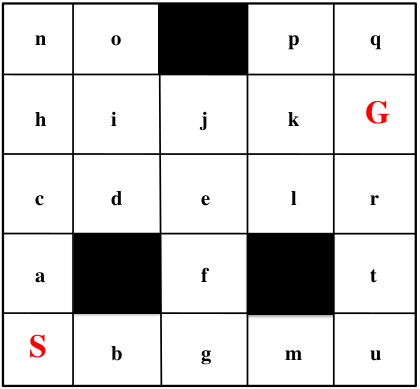
\includegraphics[width=\textwidth]{figures/l13/example-grid.png}
\end{column}
\end{columns}
\end{frame}

\begin{frame}{Toy Example}{Encoding Shortest Paths}
\begin{columns}[T]
\begin{column}{0.7\textwidth}
Basic Encoding Idea: One Boolean variable per unblocked square\\[1ex]
\begin{itemize}\itemsep1ex
	\item $S$, $G$ must be visited (hard unit clauses)
	\item All other squares: ``Prefer not to visit'' (soft unit clauses with weight 1)
\end{itemize}~\\
MaxSAT minimizes the number of visited squares.\\[1ex]
Without further constraints that formulation only visits $S$ and $G$.
\end{column}
\begin{column}{0.29\textwidth}
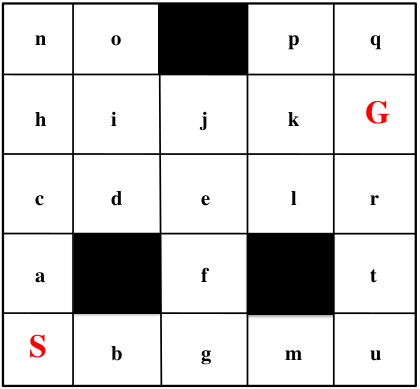
\includegraphics[width=\textwidth]{figures/l13/example-grid.png}
\end{column}
\end{columns}
\end{frame}

\begin{frame}{Toy Example}{Encoding Shortest Paths}
Ensure a valid path between $S$ and $G$.~\\[1em]
\begin{columns}[T]
\begin{column}{0.7\textwidth}
\textbf{Constraint 1:} $S$ and $G$ must have exactly one visited neighbor~\\[1ex]
\visible<2->{\begin{itemize}\itemsep1ex
	\item For $S$: $a + b = 1$ \quad CNF: $\{a, b\}, \{\lnot a, \lnot b\}$
	\item For $G$: $k + q + r = 1$ \quad CNF: $\{k, q, r\}, \{\lnot k, \lnot q\}, \{\lnot k, \lnot r\}, \{\lnot q, \lnot r\}$
\end{itemize}~\\}
\textbf{Constraint 2:} All other visited squares must have exactly two visited neighbors~\\[1ex]
\visible<2->{\begin{itemize}\itemsep1ex
	\item Example: for square $e$, if $e$ is visited, then $d + j + l + f = 2$
	\item Requires encoding a cardinality constraint in CNF
\end{itemize}}
\end{column}
\begin{column}{0.29\textwidth}
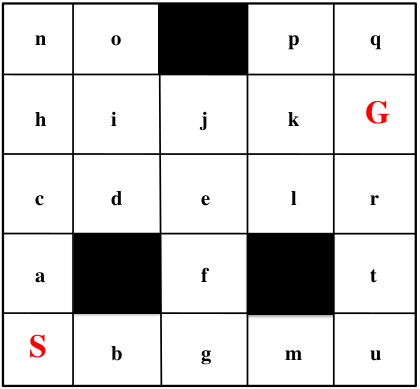
\includegraphics[width=\textwidth]{figures/l13/example-grid.png}
\end{column}
\end{columns}
\end{frame}

\begin{frame}{Toy Example}{Encoding Shortest Paths}
Path Properties: 
Every solution to the hard clauses defines a valid path from $S$ to $G$.~\\[1ex]
\begin{columns}[T]
\begin{column}{0.7\textwidth}
\begin{itemize}\itemsep1ex
	\item Each visited square falsifies a soft clause (e.g., $\lnot x$)
	\item MaxSAT solution is a shortest path (minimum number of visited squares)
\end{itemize}~\\[1em]
Example: Two valid paths from $S$ to $G$.\\[1ex]
\begin{itemize}\itemsep1ex
	\item Orange path: 14 visited squares
	\item Green path: 8 visited squares (optimal)
\end{itemize}
\end{column}
\begin{column}{0.29\textwidth}
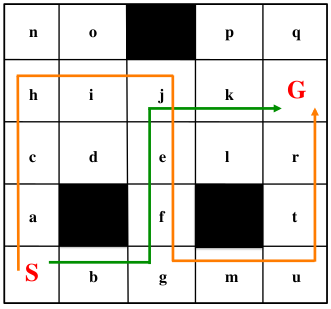
\includegraphics[width=\textwidth]{figures/l13/example-grid-sol.png}
\end{column}
\end{columns}
\end{frame}

\begin{frame}{Representing High-Level Soft Constraints}
MaxSAT can represent high-level soft constraints compactly.\\[1em]
\begin{block}{Softening an $\mathcal{NP}$-Constraint}
\begin{itemize}\itemsep1em
  \item Let $\mathcal{C}$ be a finite-domain soft constraint with weight $W_{\mathcal{C}}$
  \item Encode $\mathcal{C}$ into CNF: $CNF(\mathcal{C}) = C_1 \wedge C_2 \wedge \dots \wedge C_m$
  \item Introduce fresh variable $a$, add hard clauses: $(C_i \vee a)$ for all $i$
  \item Add soft clause: $(\lnot a)$ with weight $W_{\mathcal{C}}$
\end{itemize}
\end{block}
\end{frame}

\begin{frame}{A Glimpse into the Polynomial Hierarchy}
{Defining complexity beyond $\mathcal{NP}$}
\begin{blueblock}{Definition: Polynomial Hierarchy (without co-$\mathcal{NP}$)}
\begin{itemize}\itemsep1ex
	\item $\Sigma_0^p := \Delta_0^p := \mathcal{P}$
	\item $\Sigma_{k+1}^p = \mathcal{NP}^{\Sigma_k^p}$ \hfill (nondeterministic poly-time \emph{with} a $\Sigma_k^p$ oracle)
	\item $\Delta_{k+1}^p = \mathcal{P}^{\Sigma_k^p}$ \hfill (deterministic poly-time \emph{with} a $\Sigma_k^p$ oracle)
	\item $\mathcal{P} ~\subseteq~ \mathcal{NP} ~\subseteq~ \Delta_2^p ~\subseteq~ \Sigma_2^p ~\subseteq~ \dots ~\subseteq~ \mathrm{PH} ~\subseteq~ \mathrm{PSPACE}$
\end{itemize}
\end{blueblock}~\\
\begin{itemize}\itemsep1ex
	\item Level 1:~ $\Sigma_1^p = \mathcal{NP}$,\quad $\Delta_1^p = \mathcal{P}$
	\item Level 2:~ $\Sigma_2^p = \mathcal{NP}^{\mathcal{NP}}$,\quad \highlo{$\Delta_2^p = \mathcal{P}^{\mathcal{NP}}$}
	\item \highlo{$\Delta_2^p$} $\longleftarrow$ deciding things is as easy as polynomially many calls to an $\mathcal{NP}$ oracle (\highlo{MaxSAT})
\end{itemize}~\\[2em]
Note that the slides leave out co-$\mathcal{NP}$ to simplify the depiction: $\Pi_0^p = \mathcal{P}$, $\Pi_1^p = \text{co-}\mathcal{NP}$, $\Pi_2^p = \text{co-}\mathcal{NP}^{\mathcal{NP}}$, \dots
\end{frame}

\begin{frame}{Practical MaxSAT Solving}{Input Format, Solvers}
\begin{block}{Standard Solver Input Format: DIMACS WCNF}
\begin{itemize}\itemsep1em
	\item Like DIMACS CNF: Variables indexed from $1$ to $n$, Negation: $-i$ means $\lnot x_i$, Clauses terminated with $0$
	\item Header line: \texttt{p wcnf <\#vars> <\#clauses> <top>}
	\item Clause weight is first integer in line; if weight $\geq$ \texttt{top} $\rightarrow$ hard clause
\end{itemize}
\end{block}
\begin{block}{Push-Button Solvers / Black-box Solvers}
\begin{itemize}\itemsep1em
	\item Input: in standard WCNF format
	\item Output: provably optimal solution or \texttt{UNSATISFIABLE}
	\item Internally rely on CDCL SAT solvers to prove unsatisfiability of subsets of clauses
	\item Find recent MaxSAT solvers and benchmarks at \url{https://maxsat-evaluations.github.io/2026/}
\end{itemize}
\end{block}
\end{frame}

\begin{frame}{Recap.}
\begin{block}{So far: MaxSAT}
	\begin{itemize}\itemsep1em
		\item Powerful paradigm for Boolean optimization
		\item Wide range of real-world problems
		\item Complexity: $\Delta_2^p$-complete
		\item Standard input format: DIMACS WCNF
		\item Push-button solvers are available and effective
	\end{itemize}
\end{block}
\begin{block}{Next up}
	Fundamental algorithms for solving MaxSAT
\end{block}
\end{frame}

\begin{frame}{Algorithms for MaxSAT Solving}
\begin{block}{Example Implementations / Historic Solvers}
\begin{itemize}\itemsep1em
	\item \textbf{Branch and Bound:} MaxSatz, ahmaxsat
	\item \textbf{Direct Integer Programming:} IP Encoding + IP Solver (e.g., CPLEX, Gurobi)
	\item \textbf{Iterative, Linear SAT to UNSAT (LSU):} QMaxSAT
	\item \textbf{Core-Guided:} Eva, MSCG, OpenWBO, WPM, maxino
	\item \textbf{IP-SAT Hybrids:} MaxHS, LMHS
\end{itemize}
\end{block}
\end{frame}

\begin{frame}{Branch and Bound}{Classic method for optimization over search trees}
\begin{columns}[T]
\begin{column}{0.69\textwidth}
Effective on small, combinatorially hard problems (e.g., Max-Clique),\\
but scalability issues with thousands of variables\\[1em]
\begin{itemize}\itemsep1em
	\item UB = Maintain upper bound (UB) on current best solution cost
	\item mincost(n) = minimum cost achievable under node n
	\item Backtrack if $mincost(n) \geq UB$\\
	$\rightarrow$ no solution under node $n$ can improve the current best solution UB
\end{itemize}~\\

Basic technique:\\[1ex]
\begin{itemize}\itemsep1em
	\item Compute lower bound (LB) such that mincost(n) $\geq$ LB
	\item If LB $\geq$ UB, then backtrack ($\Rightarrow $ mincost(n) $\geq$ LB $\geq$ UB)
\end{itemize}
\end{column}
\begin{column}{0.3\textwidth}
	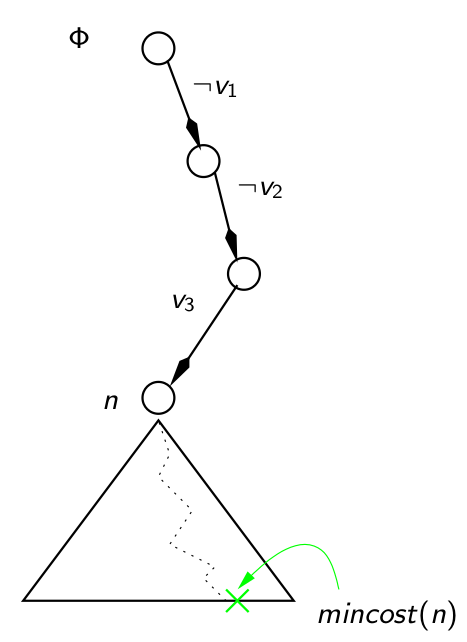
\includegraphics[width=\textwidth]{figures/l13/branchnbound.png}
\end{column}
\end{columns}
\end{frame}

\begin{frame}{Branch and Bound}{Lower Bounds by UNSAT Cores}
Look for inconsistencies that force some soft clause to be falsified.\\[1em]
\begin{itemize}\itemsep1em
	\item Strategy: find UNSAT cores, i.e. unsatisfiable subsets of clauses\\
	$\longrightarrow$ At least one clause in an UNSAT core has to be falsified
	\item Example: $\kappa = \{(\{x\},2), (\{\lnot x\}, 3)\}$ is UNSAT core\\[1ex]
	\begin{itemize}\itemsep1em
		\item replace it with $\kappa' = \{(\emptyset, 2), (\{\lnot x\}, 1)\}$
		\item Cost of $\emptyset$ (=minimum cost) gets increased by 2\\
			$\longrightarrow$ 2 is a lower bound
		\item The cost of each truth assignment is preserved
	\end{itemize}
	\item Repeat:\\[1ex]
	\begin{enumerate}\itemsep1ex
		\item Detect unsatisfiable core $\kappa$
		\item Apply sound transformation to increase $\text{cost}(\emptyset)$
		\item Stop if no further LB improvement possible or LB $\geq$ UB
	\end{enumerate}
\end{itemize}
\end{frame}

\begin{frame}{MaxSAT by Integer Programming (IP)}{Using IP solvers as MaxSAT engines}
\begin{itemize}\itemsep1ex
	\item IP solvers are widely used in Operations Research (IBM CPLEX, Gurobi, SCIP, etc.)
	\item Solve problems with linear constraints and integer variables
	\item Very effective on many standard optimization problems\\[1ex]
	Do not dominate native MaxSAT solvers on ``very Boolean'' problems
\end{itemize}~\\
\begin{block}{MaxSAT Encoding into IP}
\begin{enumerate}
	\item Relax each soft clause $C_i$ using a new variable $r_i$
	\item Convert each clause to linear constraint:
	\[
	r_i + x + (1 - y) + z + (1 - w) \geq 1
	\]
	\item Boolean variables become 0-1 bounded integers
	\item Objective function:
	\[
	\min \sum_{C_i \in F_s} w_i \cdot r_i
	\]
\end{enumerate}
\end{block}
\end{frame}

\begin{frame}{SAT-Based MaxSAT Solving}{The most widely used modern approach}
\begin{itemize}\itemsep1ex
	\item Solve a sequence of SAT instances that ask for different values of $k$:
	\begin{quote}
	Is there a truth assignment falsifying at most $k$ soft clauses?
	\end{quote}
	\item SAT-based MaxSAT algorithms mainly do two things:\\[1ex]
	\begin{enumerate}\itemsep1em
	\item Develop better ways to encode this decision problem.Algorithms for solving MaxSAT
\
	\item Find ways to exploit information obtained from the SAT solver at each stage in the next stage.
	\end{enumerate}
\end{itemize}~\\
Assume unit-weight soft clauses for now \dots

\begin{block}{Methods for SAT-Based MaxSAT}
\begin{itemize}\itemsep1em
  \item \textbf{Iterative Search:} Iteratively increase (decrease) $k$ until SAT (UNSAT)
  \item \textbf{Core-Based Methods:} Use unsatisfiable cores to guide search
  \item \textbf{Hybrid Methods:} Combine SAT solving with integer programming
\end{itemize}
\end{block}
\end{frame}

\begin{frame}{Iterative Search}
\vspace{-2em}
To check whether F has a solution of cost $\leq k$, solve: $(C_1 \vee r_1) \wedge \cdots \wedge (C_n \vee r_n) \wedge \left(\sum_{i=1}^n r_i \leq k\right)$, and iterate over $k = 1, 2, \dots$ until optimal $k$ is found.\\[1ex]
\begin{block}{Iterating over $k$}
	\begin{itemize}\itemsep1ex
		\item \textbf{Linear Search (UNSAT to SAT):} (not efficient)\\
		Start at $k = 1$, increment until SAT
		\item \textbf{Linear Search (SAT to UNSAT):} (can be effective)\\
		\begin{itemize}
			\item Find model $\pi$ for hard clauses, let $k = \#$violated soft clauses$-1$
			\item Try solving again with lower $k$ until UNSAT
			\item If SAT: set $k$ to $\#$violated soft clauses and repeat
			\item If UNSAT: last SAT solution is optimal
		\end{itemize}
		\item \textbf{Binary Search:} (can be effective with core-based reasoning)\\
		\begin{itemize}
			\item Initialize: $LB = 0$, $UB = \#$soft clauses
			\item Check $k = \lfloor \frac{LB + UB}{2} \rfloor$
			\item If SAT: $UB = k$, else $LB = k + 1$
			\item Stop when $UB = LB + 1$, then UB is optimal.
		\end{itemize}
	\end{itemize}
\end{block}
\end{frame}

\begin{frame}{SAT-Based MaxSAT Solving using UNSAT Cores}
\vspace{-2em}
\begin{block}{Motivation}
Adding linear cardinality constraints over all soft clauses is too loose:
\begin{itemize}\itemsep1ex
	\item One relaxation variable $r_i$ per soft clause, could be well over 100k of variables
	\item Linear cardinality constraints over all soft clauses are too loose:\\
	no information about which relaxation variables to assign to 1
	\item SAT solver must explore many subsets of soft clauses
\end{itemize}
\end{block}
\begin{block}{Unsatisfiable Cores in MaxSAT}
Core-based approach gives more powerful constraint over which particular soft clauses to relax.
\begin{itemize}\itemsep1ex
	\item \textbf{UNSAT Core:} A subset $F'_s \subseteq F_s$ s.t. $F_h \wedge F'_s$ is UNSAT
	\item At least one clause in each core must be falsified
	\item Instead of iteratively ruling out non-optimal solutions, iteratively find and rule out UNSAT cores
	\item Typically cores are much smaller than full soft clause set
\end{itemize}
\end{block}
\end{frame}

\begin{frame}{Core-Guided MaxSAT Algorithms: Fu-Malik}{The Original}
\begin{itemize}\itemsep1em
	\item First core-guided MaxSAT algorithm [Fu \& Malik, 2006]
	\item Iterative approach:
	\begin{enumerate}\itemsep1ex
		\item Find an UNSAT core
		\item Relax clauses in the core with new variables
		\item Add an AtMost-1 constraint over new relaxation vars
	\end{enumerate}
	\item Repeat until the formula becomes SAT
	\item Each iteration lowers the cost of solutions by 1 (in the unweighted case)
\end{itemize}
\end{frame}

\begin{frame}{Fu-Malik: Example}
\vspace{-2em}
\begin{itemize}\itemsep1em
	\item Initial Formula:\\
	$\begin{array}{lllll}
	C_1 = x_6 \vee x_2, 
	&C_2 = \lnot x_6 \vee x_2, 
	&C_3 = \lnot x_2 \vee x_1, 
	&C_4 = \lnot x_1, 
	&C_5 = \lnot x_6 \vee x_8,\\
	C_6 = x_6 \vee \lnot x_8, 
	&C_7 = x_2 \vee x_4, 
	&C_8 = \lnot x_4 \vee x_5, 
	&C_9 = x_7 \vee x_5, 
	&C_{10} = \lnot x_7 \vee x_5,\\
	C_{11} = \lnot x_5 \vee x_3, 
	&C_{12} = \lnot x_3
	\end{array}$
	\item Core 1: $\{C_3, C_4, C_7, C_8, C_{11}, C_{12}\}$
	\item Add relaxation variables $r_1$ to $r_6$, and AMO constraint $\sum r_i \leq 1$
	\item Core 2: $\{C_1, C_2, C_3, C_4, C_9, C_{10}, C_{11}, C_{12}\}$
	\item Add relaxation variables $r_7$ to $r_{14}$ to these clauses, and AMO constraint $\sum_{i=7}^{14} r_i \leq 1$
	\item Now the instance is SAT, and the optimal cost is the number of iterations (2 here)
	\item Final Formula:\\
	$\begin{array}{lllll}
	C_1 = x_6 \vee x_2 \vee r_7, 
	&C_2 = \lnot x_6 \vee x_2 \vee r_8, 
	&C_3 = \lnot x_2 \vee x_1 \vee r_1 \vee r_9, 
	&C_4 = \lnot x_1 \vee r_2 \vee r_{10}, 
	&C_5 = \lnot x_6 \vee x_8\\
	C_6 = x_6 \vee \lnot x_8, 
	&C_7 = x_2 \vee x_4 \vee r_3, 
	&C_8 = \lnot x_4 \vee x_5 \vee r_4, 
	&C_9 = x_7 \vee x_5 \vee r_{11}, 
	&C_{10} = \lnot x_7 \vee x_5 \vee r_{12}\\
	C_{11} = \lnot x_5 \vee x_3 \vee r_5 \vee r_{13},
	&C_{12} = \lnot x_3 \vee r_6 \vee r_{14},
	&\sum_{i=1}^{6} r_i \leq 1,
	&\sum_{i=7}^{14} r_i \leq 1
	\end{array}$
\end{itemize}
\end{frame}

\begin{frame}{Other Core-Guided MaxSAT Algorithms}
\vspace{-2em}
\begin{block}{MSU3 Algorithm by Marques-Silva and Planes (2007)}
Differences to Fu-Malik:
\begin{itemize}
	\item Introduce only at most one relaxation variable to each soft clause\\
	$\rightarrow$ Re-use already introduced relaxation variables
\end{itemize}
\end{block}
\begin{block}{OpenWBO Algorithm by Martins, Joshi, Manquinho, and Lynce, 2014}
Combines MSU3 with incremental construction of the cardinality constraint:\\
$\rightarrow$ Each new constraint builds on the encoding of the previous constraint
\end{block}
\begin{block}{WPM2 Algorithm by Ansótegui, Bonet, and Levy, 2013a}
Proposes a method for dealing with overlapping cores: groups intersecting cores into disjoint covers.\\
The cores might not be disjoint but the covers will be\\
$\rightarrow$ at-most-k constraints over the soft clauses in a cover\\
$\rightarrow$ at-least-k constraint over the clauses in a core
\end{block}
\end{frame}

\begin{frame}{Implicit Hitting Set Algorithms for MaxSAT}{Combining Integer Programming with SAT solving}
\begin{block}{Hitting Sets}
Given a collection of sets $\mathcal{S}$ of elements, a \textbf{hitting set} $H$ is a subset of elements that intersects all sets $S \in \mathcal{S}$.\\
A hitting set $H$ is optimal if no smaller hitting set exists.\\[1em]
\textbf{Relationship to MaxSAT:}
For any optimal hitting set $H$ of the set of UNSAT cores of a formula $F$,\\
there is an optimal solutions $\tau$ to $F$ such that $\tau$ satisfies exactly the clauses $F \setminus H$.\\[1em]
\textbf{Key Insight:}
To find an optimal solution to a MaxSAT instance $F$, it suffices to:\\[1ex]
\begin{enumerate}
	\item Find an (implicit) hitting set $H$ of the UNSAT cores of $F$.\\
	$\rightarrow$ Implicit refers to not necessarily having all MUSes of $F$.
	\item Find a solution to $F \setminus H$.
\end{enumerate}
\end{block}
\end{frame}

\begin{frame}{Implicit Hitting Set Algorithms for MaxSAT}
\begin{block}{Hitting Set Problem as Integer Programming}
$$
\min\sum_{C \in \bigcup \mathcal{K}} c(C) \cdot r_C \quad \text{subject to} \quad \sum_{C \in \mathcal{K}} r_C \geq 1 \quad \forall K \in \mathcal{K}
$$
\begin{itemize}\itemsep1ex
	\item $r_C = 1$ iff clause $C$ is in the hitting set
	\item Weight function $c$: works also for weighted MaxSAT
\end{itemize}
\end{block}
\begin{block}{MaxSAT Solving with Implicit Hitting Sets}
Iterate over the following steps:\\[1ex]
\begin{itemize}\itemsep1ex
	\item Accumulate a collection $\mathcal{K}$ of UNSAT cores
	\hfill (using a SAT solver)
	\item Find an optimal hitting set $H$ over $\mathcal{K}$,\\ 
	and rule out the clauses in $H$ for the next SAT solver call
	\hfill (using an IP solver)
\end{itemize}~\\
\dots until the SAT solver returns a satisfying assignment.
\end{block}
\end{frame}

\begin{frame}{Implicit Hitting Set Algorithms for MaxSAT}{Optimizations}
\begin{block}{Optimizations}
\begin{itemize}
	\item a disjoint phase for obtaining several cores before/between hitting set computations
	\item combinations of greedy and exact hitting sets computations
	\item \dots
\end{itemize}
Some of these optimizations are integral for making the solvers competitive.\\
\end{block}~\\
\begin{block}{IHS MaxSAT Solvers}
For more on some of the details, see
\begin{itemize}
	 \item \textbf{MaxHS} [Davies and Bacchus, 2011 and 2013]
	 \item \textbf{LMHS} [Saikko, Berg, and Järvisalo, 2016]
\end{itemize}~\\
IHS Algorithms for MaxSAT are among the best performing solvers today, and work well on a wide range of problems, particularly on large instances with many different weights on soft clauses.
\end{block}
\end{frame}

\end{document}
